\chapter{Souborové systémy OS Linux}
%\todo{Srovnani ext3, ext4, udf, fat, ntfs, ... a nastroju pro ně, soustředit se na fsck}
%\todo{Vysvětlit co to je souborový systém?}

\section{Fyzická úložná média}
%\todo{Ozdrojovat...}
Fyzická úložná média představují nejnižší vrstvu  a zároveň základní kámen všech souborových systémů, protože právě na základě jejich vlastností byly vytvářeny.\\
Z historického hlediska po současnost vývoj přešel přes několik technologií počínaje děrnou páskou a děrnými štítky přes magnetické ukládáním informace do různých nosných médií, optická média po flash paměti. Z hlediska souborových systémů má smysl mluvit až o magnetických médiích, která byla použita pro běžnou práci, protože například lineární pásková úložiště nebyly konstruovány pro kompatibilitu s ostatními systémy ale pouze pro vlastní potřeby, tudíž záznam neobsahoval metadata ale pouze data samotná a jejjich struktura byla uložena jinde nebo vůbec. První opravdové použití souborového systému přišlo až s nástupem disket a pevných disků. \\
První opravdový souborový systém v Unixu byl \textbf{S5FS} neboli \emph{System V File System} (1974), často ovšem označovaný pouze jako \textbf{FS} (File System) nebo \textbf{UFS} (Unix File System) který byl implementován v \emph{UNIX System V} běžící například na mainframech PDP-11. Tento souborový systém byl velice pomalý a také poměrně jednoduchý, ale právě jeho architektura posloužila jako vzor většiny následujících unixových souborových systémů. Tomu ovšem předcházel souborový systém pro mikropočítače s názvem \textbf{CP/M} (1973) neboli \emph{Control Program/Monitor} a později \emph{Control Program for Microcomputer}. Tento souborový systém byl určen narozdíl od S5FS pro mikropočítače od společnosti Intel. V době vzniku totiž začal Intel vyrábět první osmibitové procesory Intel 8008 a o rok později v roce 1974 vznikl Intel 8080 a právě s ním se rozšířil i CP/M. CP/M byl někde na pomezí mezi souborovým a operačním systémem. Na úložném médiu (v tomto případě disketě) byl BIOS, který poskytoval systémová volání na zápis a čtení, řízení klávesnice a monitoru. Poté bylo CP/M, které využívalo těchto volání a poskytovalo je spolu s dalšími shellu a uživatelskému programu. Systémová volání které přidalo CP/M se týkaly převážně přístupu k souborům, která CP/M uchovávalo. Dalším významným souborouvým systémem, který vznikl pro diskety byl \textbf{FAT12} (1977). Posléze s rozšířením pevných disků se začaly vyvíjet další nové souborové systémy odpovídající požadavkům.\\
Z hlediska struktury disku lze mluvit o CHS (Cylinder Head Sector), které rozdělilo úložné médium ve třech rozměrech podle jednotlivých stop (Cylinder), čtecí hlavy (Head), kterých může být u pevných disků více, záleží na počtu jednotlivých disků a použitých stran a poslední rozměr je sektor (Sector), který určuje o kterou část stopy jde. Právě sektory dostály ve vývoji největších změn, protože původní dělení po úhlech od středu disku nebylo efektivní se vzrůstající vzdáleností od středu. Proto se později přešlo k dělení na jednotnou velikost sektoru, které se rozložily rovnoměrně po celém disku.\\
Sektor je nejmenší zápisovou jednotkou na médiu, která je určená výrobcem média. Typicky se jedná o velikosti 512~B u pevných disků, 2048~B u CD-ROM a DVD-ROM. Nové pevné disky používají velikost bloku 4096~B. Důvodem pro členění po sektorech je zjednodušení přístupu k médiu za předpokladu, že uložená data jsou větší než velikost bloku. V opačném případě dochází k plýtvání místem, protože se vždy čte a zapisuje celý blok. Právě proti sektorům se obvykle navrhují bloky souborového systému, které se snaží využít sektory co nejefektivněji jak z hlediska úspory místa tak z hlediska přístupového a zápisového času.

\section{Diskové oddíly}
Diskové oddíly představují způsob, jak lze fyzické médium abstraktně rozdělit na více částí. Rozdělení na oddíly je uloženo v MBR (Master Boot Record) a jeden disk může obsahovat až 4 hlavní oddíly. V případě potřeby více oddílů lze použít rozšířený oddíl, který zapouzdřuje další dělení na oddíly, ovšem tentokrát již mimo MBR.\\
Důvodem pro rozdělení na oddíly může být oddělení uživatelských dat od systémových, vyhrazení místa pro odkládací oddíl nebo jiné logické dělení. 

\section{Logical Volume Manager (LVM)}
%\todo{https://wiki.archlinux.org/index.php/LVM}
Logical Volume Manager (LVM) představuje způsob abstrakce nad diskovými oddíly. Ačkoli se může zdát, že se jedná o podobnou technologii jako je RAID, není tomu tak (\cite{arch-lvm}).\\
LVM vzniklo pro zajištění větší flexibility pro organizaci úložiště. Představte si situaci na následujícím obrázku:
\pagebreak
\begin{verbatim}
Disk1 (/dev/sda):
 _ _ _ _ _ _ _ _ _ _ _ _ _ _ _ _ _ _ _ _ _ _ _ _ _ _ _ _ _ _ _ _ _ _ _ _ _
|Partition1 50GB (Physical volume) |Partition2 80GB (Physical volume)     |
|/dev/sda1                         |/dev/sda2                             |
|_ _ _ _ _ _ _ _ _ _ _ _ _ _ _ _ _ |_ _ _ _ _ _ _ _ _ _ _ _ _ _ _ _ _ _ _ |
                                                     
Disk2 (/dev/sdb):
 _ _ _ _ _ _ _ _ _ _ _ _ _ _ _ _ _ _ _ _ _ _ _ _ _ _
|Partition1 120GB (Physical volume)                 |
|/dev/sdb1                                          |
| _ _ _ _ _ _ _ _ _ _ _ _ _ _ _ _ _ _ _ _ _ _ __ _ _|
\end{verbatim}
Jak je vidět, situace obsahuje dva disky, každý o jiné velikosti a formátu. Pokud bychom chtěli vytvořit diskový oddíl, museli bychom sáhnout po řešení RAID 0 a disky posléze naformátovat dle potřeby. V případě změny velikosti by bylo nutné uložiště přeformátovávat. Ovšem při použití LVM situace vypadá například takto:
\begin{verbatim}
Volume Group1 (/dev/MyStorage/ = /dev/sda1 + /dev/sda2 + /dev/sdb1):
 _ _ _ _ _ _ _ _ _ _ _ _ _ _ _ _ _ _ _ _ _ _ _ _ _ _ _ _ _ _ _ _ _ _ _ _ _ 
|Logical volume1 15GB  |Logical volume2 35GB    |Logical volume3 200GB    |
|/dev/MyStorage/rootvol|/dev/MyStorage/homevol  |/dev/MyStorage/mediavol  |
|_ _ _ _ _ _ _ _ _ _ _ |_ _ _ _ _ _ _ _ _ _ _ _ |_ _ _ _ _ _ _ _ _ _ _ _ _|
\end{verbatim}
Všechny oddíly byly sloučeny do jedné logické skupny s názvem \texttt{MyStorage} s velikostí 250~GB a to bylo následně pouze logicky rozděleno na oddíly jak je vidět na obrázku. Tyto logické oddíly posléze budou naformátovány libovolným souborovým systémem.\\
Zásadní rozdíl oproti RAID 0 je v možnostech změny struktury úložiště. V případě RAID 0 se změna promítá do formátování RAID úložiště, v případě LVM se jedná o změnu velikosti logické jednotky pouze za předpokladu existence nějakého volného místa, nezávisle na jeho místě na disku. Tudíž není třeba přesouvat oddíly pro potřeby jejich zvětšení.

\section{Srovnání souborových systémů}
Pro operační systém Linux bylo během jeho existence vyvinuto mnoho různých souborových systémů stejně tak jako jich bylo mnoho implementováno z ostatních operačních systémů. Některé z nich jsou používány i v současnosti, některé byly opuštěny nebo nahrazeny.\\
Podle \cite{tldp-filesystem} patří mezi nejvýznamnější nativní souborové systémy tyto:
\begin{itemize}
    \item \textbf{ufs} -- \todo{popsat UFS}
    \item \textbf{minix} -- nejstarší souborový systém OS Linux. Vzhledem k jeho stáří se dnes již aktivně nevyvíjí a nepoužívá. Mezi jeho hlavní omezení patří maximální velikost souborového systému, která je až 64~MB. Dalším významným omezením je délka názvů souborů, která je limitována na 30 znaků.
    \item \textbf{ext} -- tento souborový systém, celým jménem Extended Filesystem, vznikl v roce 1992 speciálně pro potřeby kernelu OS Linux \cite{linmag-ext}. Jeho inspirací byl souborový systém UFS (Unix File System), ze kterého převzal strukturu metadat. Jeho limitací byla maximální velikost 2~GB.
    \item \textbf{ext2} -- nástupce souborového systému ext. Byla navýšena maximální velikost na 32~TB a byl navržen podle stejných principů jako Berkeley Fast File System z projektu BSD \cite{nongnu-ext2}. Dlouhou dobu byl tento souborový systém používán ve všech hlavních distribucích OS Linux. ext2 nebyl zpětně kompatibilní s původním ext.
    \item \textbf{ext3} -- již v pořadí třetí verze ext souborového systému. Nyní již byla zachována téměř plná zpětná kompatibilita s ext2. Oproti ext2 ovšem ext3 přineslo žurnálování, které pomohlo v obnově souborového systému při chybě systému \cite{paper-ext3}. Zbytek parametrů zůstal shodný s ext2.
    \item \textbf{ext4} -- současná verze ext souborového systému \cite{paper-ext4}. Opět je zpětně kompatibilní s ext3 a ext2 ale oproti nim byla navýšena maximální velikost na 1~EB, ale doporučené maximum je 16~TB. Původně byl ext4 pouze skupina rozšížení pro ext3, ale později se osamostatnil jako ext4. Dalším rozšířením je nyní již neomezený počet podsložek (ext3 mělo omezení na 32000 podsložek). Také bylo zlepšena odolnost žurnálu přidáním kontrolních součtů a celková výkonnost souborového systému.
    \item \textbf{vfat} -- typický zástupce cizích souborových systémů. V tomto případě se jedná o MS FAT32, který je hojně používaný na USB flash discích.
    \item \textbf{iso9660} -- standardní souborový systém pro CD-ROM. 
    \item \textbf{udf} -- souborový systém původně vyvynutý pro datové rozšíření CD-ROM. Posléze rozšířen pro DVD a BluRay. V současnosti je používán například v šifrovaných flash discích. 
    \item \textbf{smbfs} -- síťový souborový systém Samba File Systém vyvinutý pro sdílení dat mezi počítači s MS Windows. Podporuje Windows Sharing Protocol.
    \item \textbf{ntfs} -- v současnosti nejpoužívanější souborový systém v MS Windows. \todo{MORE}
    \item \textbf{btrfs} -- \todo{???}
    \item \textbf{appfs} -- \todo{???}
\end{itemize}

\section{Nástroje kontroly integrity}
V prostředí OS Linux je pro kontrolu integrity určen primárně nástroj \texttt{fsck} (Filesystem Consistency Check). V manuálové stránce k \texttt{fsck} \cite{man-fsck} se lze dočíst, že samotný \texttt{fsck} je pouze frontend, který volá specifické nástroje pro daný souborový systém. Skutečné nástroje určené pro kontrolu integrity, které jsou obvykle dodávány spolu s nástroji k vytvoření a práci s daným soborovým systémem se jmenují \texttt{fsck.fstype}, například \texttt{fsck.ext4}.\\
Pro masivně používané souborové systémy tyto nástroje existují. Pro \textbf{ext} rodinu se jedná o nástroj \texttt{e2fsck}. Podporovány jsou i převzaté souborové systémy, například \texttt{fsck.fat} pro souborové systémy \textbf{vfat} a \textbf{msdos}. Ovšem pro například pro \textbf{iso9660} nástroje kontrolující integritu existují pouze jako nástroje vzniklé na základě pokusů při testování vadných disků. Takovým je i \texttt{isovfy} \cite{man-isovfy} ze skupiny nástrojů isoinfo, který ovšem pouze umožňuje kontrolu integrity, nikoli opravu chyb.\\
Nástrojem který v tuto chvíli chybí je podle všeho \texttt{fsck.udf}. Projekt s názvem udftools \cite{udftools-sourceforge} ve kterém vznikl i podprojekt udffsck byl autorem opuštěn v roce 2004 a nástroj pro kontrolu konzistence nebyl nikdy započat a proto se v dalších částech práce soustředím právě na tento souborový systém. 

\chapter{Universal Disk Filesystem}
\label{sec:udf}
%\todo{Popsat filesystem, způsob uložení dat, ochrané mechanismy... UDF docs rulez!}
Universal Disk Filesystem (UDF) je souborový systém navržený pro použití na CD, DVD a Blu-Ray discích, ale díky jeho univerzálnosti je možné jej použít i na jiných médiích. Jeho návrh vyšel ze systému CDFS (ISO 9660) ale není s ním kompatibilní. Jednou z výhod UDF oproti CDFS je například možnost dodatečného zápisu na CD anebo naopak mazání dat z CD a přepisovatelných disků.
\todo{Popsat klíčové vlastnosti UDF}
\section{Historie UDF}
\todo{revize, standardy, erraty}

\section{Struktura systému}
Norma popisující UDF definuje dva druhy číslování. Prvním je \textit{Logical Sector Number} (LSN), které popisuje čísla jednotlivých sektorů. Je číslované od nuly a začíná na prvním fyzickém sektoru média. Jeho velikost by měla odpovídat fyzické velikosti sektoru. Jeho určením je fyzická navigace na médiu. Druhým je \textit{Logical Block Number} (LBN), které popisuje čísla jednotlivých logických bloků, které jsou mapovány na sektory. Jejich velikost by měla být stejná jako velikost LSN. Jsou číslované od nuly ale začínají až v oblasti dat. Jeho určením je na rozdíl od LSN navigace pouze v datech.\\
\todo{Zmatečné, přepsat}
Samotný FS je rozdělen do pěti částí. První je \textit{Volume Recognition Sequence} (VRS). Tato část je lokalizována na fixní adrese \texttt{0x10000}, což odpovídá sektoru 16 při velikosti sektoru 2~kB. Důvodem této fixní adresy je právě dodržení zpětné kompatibility se standardem ISO9660, který předpokládá použití pouze na optických médiích s velikostí sektoru 2~kB. Tato zpětná kompatiblita pokračuje dále v tom smyslu, že celá VRS je dále zpracovávána právě po 2~kB blocích, pokud je velikost fyzického sektoru menší nebo stejná. V opačném případě je nutné přejít k blokům větším a zpětná kompatibilita je porušena. Význam VRS je identifikace použitého souborového systému na médiu. Více o VRS je v samostané kapitole \ref{sec:vrs}.\\
\todo{Konec zmatečného}
Další částí je \textit{Anchor Volume Descriptor Pointer} (AVDP). Tato část je již pouze pro UDF a jedná se o výchozí bod při čtení souborového systému. Mají několik různých umístění a typicky je na médiu vícekrát. Obsahuje jedinou informaci a tou je umístění \textit{Volume Descriptor Sequence} (VDS) a to jak hlavní, tak záložní. Více je v kapitole \ref{sec:avdp}.\\
Následující částí je již zmíněný \textit{Volume Descriptor Sequence} (VDS). Tato skupina deskriptorů popisuje veškeré vlastnosti souborového systému, jeho stav a další. Je zaznamenána vždy ve dvou exemplářích pro zvýšení robustnosti. VDS je detailněji popsána v kapitole \ref{sec:vds}.\\
Další částí je \textit{Logical Volume Integrity Descriptor} (LVID), který popisuje integritu souborového systému. Více je v kapitole \ref{sec:lvid}. Tímto deskriptorem končí metadata systému.\\
\todo{obrazek}
Poslední částí jsou samotná data. Jejich výchozím bodem je \textit{File Set Descriptor} (FSD), který udržuje informaci o počtu adresářů a souborů a umístění kořenového adresáře. Poté následují už samotné deskriptory dat následované daty.\\
Vzhledem k možné koexistenici s ISO9660 na médiu je možné že budou existovat i struktury tohoto souborového systému. Tuto skutečnost je potřeba mít na paměti při případném zápisu dat na médium. Pro samotné čtení není třeba se nad touto skutečností déle pozastavovat.

\section{Deskriptory UDF systému}
Tato část stručně popisuje skupiny deskriptorů souborového systému UDF. Jedná se pouze o přehledovou část vzhledem k velkému překryvu specifikací, která je uvedena v \cite{osta-udf-0201} a standardem ECMA-167, který je uveden v \cite{ecma-167}.

\subsection{UDF Bridge Volume Recogniton Sequence}
\label{sec:vrs}
Tato sekce je určena k rozpoznání obsaženého souborového systému. Jak bylo předesláno v předchozí kapitole, může být velká až 6 sektorů \todo{nikde to není řečeno...} a obsahuje deskriptor identifikující souborový systém. Jeho poloha je fixní na sektoru 16. \todo{sjednotit s předchozí kapitolou. Tam je 0x10000, tady je 16...}\\
Struktura deskriptorů je zachycena v tabulce \ref{tab:vrs}.
\begin{table}
    \begin{tabular}{ | l | l | l | l | l | }
        \hline
        Adresa  & Délka [B]   & Jméno položky & Datový typ    & Popis \\ \hline
        0       & 1             & Type           & int8          & Typ deskriptoru \\ \hline
        1       & 5             & Identifier & string        & Identifikátor typu souborového systému \\ \hline
        6       & 1             & Version         & int8          & Verze deskriptoru \\ \hline
        7       & 2041          & ---           & ---           & Volné místo, záleží na typu deskriptoru \\ \hline
    \end{tabular}
    \caption{Struktura VRS deskriptorů\label{tab:vrs}}
\end{table}
Jak je vidět, deskriptor se skládá ze třech částí, pomineme-li poslední rezervovanou část obsahující volné místo. První položka \textit{Type} určuje typ deskriptoru. V tomto případě je jediná povolená hodnota 1. Další položka s názvem \textit{Identifier} obsahuje řetězec o pěti znacích. Tato část určuje typ použitého souborového systému. Možné varianty jsou tyto:
\begin{itemize}
    \item \texttt{BOOT0} - Bootovací záznam
    \item \texttt{CD001} - Souborový systém ISO~9660
    \item \texttt{CDW02} - Souborový systém podle ECMA-168 \cite{ecma-168}
    \item \texttt{BEA01} - \textit{Beginning Extended Area Descriptor}, začátek UDF Bridge sekvence
    \item \texttt{TEA01} - \textit{Terminating Extended Area Descriptor}, konec UDF Bridge sekvence
    \item \texttt{NSR01} - UDF verze 1.0 a vyšší
    \item \texttt{NSR02} - UDF verze 1.5 a vyšší
    \item \texttt{NSR03} - UDF verze 2.0 a vyšší
\end{itemize}
Poslední položkou je \textit{Version} která obsahuje informaci o verzi deskriptoru. Zde by měla být v těchto případech vždy \texttt{0x01}.\\
Aby mohlo být prohlášeno, že médium obsahuje UDF, musí být nalezen deskriptor obsahující \textit{Identifier} s hodnotou \texttt{NSR01}, \texttt{NSR02} nebo \texttt{NSR03}. V opačném případě se nejedná o UDF.

\subsection{Anchor Volume Descriptor Pointer}
\label{sec:avdp}
\textit{Anchor Volume Descriptor Pointer} (AVDP) je klíčová část souborového systému. Tato struktura udržuje adresu deskriptorů souborového systému a jejich délku. Právě AVDP je první deskriptor, který se čte po identifikaci souborového systému, proto je umístěn na předem známém místě. \todo{Popsat uzavřený a otevřený FS} V případě uzavřených souborových systémů to je na sektoru 256, posledním sektoru média a nezřídka také na 256 sektoru od konce média. V případě otevřených souborových systémů je zde výjimka, protože AVDP je dočasně umístěno na sektoru 512 až do uzavření systému.\\
Jeho struktura je popsána v tabulce \ref{tab-avdp}. Jak je vidět, obsahuje ukazatele na hlavní a záložní VDS což zvyšuje robustnost celého souborového systému.
\begin{table}[hb]
    \begin{tabular}{ | l | l | p{4.5cm} | p{1.3cm} | p{5.5cm} | }
        \hline
        Adresa  & Délka [B]   & Jméno položky & Datový typ    & Popis \\ \hline
        0       & 16          & DescriptorTag & struct        & Popis deskriptoru \\ \hline
        16      & 8           & MainVolumeDescriptor SequenceExtent & struct & Sektor a délka \textit{Main Volume Descriptor Sequence} \\ \hline
        24      & 8           & ReserveVolumeDescriptor SequenceExtent & struct & Sektor a délka \textit{Reserve Volume Descriptor Sequence} \\ \hline
        32      & 480         & Rezerva & & \\ \hline
    \end{tabular}
    \caption{Anchor Volume Descriptor Pointer\label{tab-avdp}}
\end{table}

\subsection{Volume Descriptor Sequence}
\label{sec:vds}
\textit{Volume Descriptor Sequence} (VDS) je skupina deskriptorů popisující veškeré vlastnosti souborového systému UDF. Jsou seřazeny postupně na jednotlivých sektorech počínaje adresou udanou z AVDP (viz. kapitola \ref{sec:avdp}) a končí po počtu logických sektorů uloženém opět v AVDP. Jsou uloženy postupně po sektorech od výchozí adresy a končí \textit{Terminating Descriptor}, což je prázdný deskriptor, který obsahuje pouze \textit{Descriptor Tag}. Samotné pořadí deskriptorů není pevné a samotné deskriptory jsou identifikovány právě pomocí \textit{Descriptor Tag}.\\
Jak je vidět v AVDP, i tato část je uložena duplicitně pro zvýšení robustnosti. Rezervní VDS je uložena ve stejném tvaru jako primární tentokrát však od jiné adresy, opět uvedené v AVDP.\\
Samotné deskriptory jsou popsány v \cite{osta-udf-0201}, kapitola 2.2. Pro kompletnost zde uvedu jejich výčet ze standardu verze 2.01.
\begin{itemize}
    \item \textit{Primary Volume Descriptor}
    \item \textit{Logical Volume Descriptor}
    \item \textit{Unallocated Space Descriptor}
    \item \textit{Implementation Use Volume Descriptor}
    \item \textit{Partition Descriptor}
    \item \textit{Terminating Descriptor}
\end{itemize}

\subsection{Logical Volume Integrity Sequence}
\label{sec:lvid}
Další důležitou částí je \textit{Logical Volume Integrity Descriptor} (LVID) spolu s \textit{Terminating Descriptor} (TE). Tato sekvence je uložena pouze jednou a její umístění je udržováno v LVD. Odpovídá na následující otázky:
\begin{itemize}
    \item Je Logický svazek v konzistentním stavu?
    \item Kdy bylo naposledy cokoli na Logickém svazku modifikováno.
    \item Kolik bloků je volných na svazku?
    \item Jaká je celková velikost svazku v blocích?
    \item Byl obsah modifikován nějakou \textit{jinou} implementací od posledního přístupu implementace která svazek vytvořila?
\end{itemize}
Jak je vidět z tohoto výčtu, tato část je důležitá hlavně pro čtení a zápis, ale i pro kontrolu dat má svůj význam, například právě kvůli informaci o konzistenci svazku.\\ 
Samotný formát struktury je opět v \cite{osta-udf-0201}, kapitola 2.2.6.

\section{File Structure}
\label{sec:fsd}
Souborová struktura UDF je postavena na třech deskriptorech, které se podílí na popisu a uložení dat. Jedná se o tyto deskriptory:
\begin{itemize}
    \item \textit{File Set Descriptor} (FSD)
    \item \textit{File Entry} (FE)
    \item \textit{File Identifier Descriptor} (FID)
\end{itemize}

\subsection{File Set Descriptor}
\label{sec:fsd}
\textit{File Set Descriptor} (FSD) je výchozím bodem pro čtení dat. Jeho pozice je opět uložena v LVD. Jeho struktura je popsána v \cite{osta-udf-0201}, kapitola 2.3.2. Tato strukutra mimo jiné obsahuje umístění kořenového adresáře. Z hlediska kontroly dat nejsou ostatní údaje tolik významné.

\subsection{File Entry}
\label{sec:fe}
\textit{File Entry} (FE) je deskriptor, který popisuje samotný soubor. Jeho pozice je určena jeho \textit{rodičem}, což v případě kořenového adresáře je FSD, ale uvedený je opět kořenový adresář, v případě ostatních souborů a adresářů se jedná o adresář, v němž se nachází.\\
Jeho struktura je popsána v \cite{osta-udf-0201}, kapitola 2.3.6, a z ní pouze vyberu některé důležité části. První důležitou informací je počet zapsaných bloků (\textit{LogicalBlocksRecorded}). Další důležitou částí jsou \textit{AllocationDescriptors}. Velikost této části je určena pomocí \textit{LengthofAllocationDescriptors} a obsahuje dva druhy dat, podle toho jestli se FE popisuje adresář nebo soubor.\\
V případě souboru je v tomto místě uložena pozice dat souboru ve formě \textit{Long Allocation Descriptor} nebo \textit{Short Allocation Descriptor}. Vždy bude použit pouze jeden z nich a měl by být uložen pouze jeden, protože data jsou ukládána sekvenčně do bloků za sebou.\\
V případě adresáře jsou v \textit{AllocationDescriptors} uloženy \textit{File Identifier Descriptor} (kapitola \ref{sec:fid}), přičemž každý jeden deskriptor nese informaci o jednom \textit{potomkovi} adresáře. Vždy je přítomen nejméně jeden FID a tím je \textit{rodičovský adresář}. 

\subsection{File Identifier Descriptor}
\label{sec:fid}
\textit{File Identifier Descriptor} (FID) je struktura, která udržuje informace o souboru na úrovni mateřského adresáře. Je popsaný v \cite{osta-udf-0201} v kapitole 2.3.4.\\
Vzhledem k faktu, že cílem této struktury není adresovat data ale jen FE, obsahuje jen metadata metadat souboru. Například jestli adresované FE popisuje složku nebo soubor, jestli je soubor smazaný nebo jestli uživatel má vědět o existenci souboru. Dále tato struktura obsahuje identifikátor souboru v podobě textového řetězce (jméno souboru nebo složky). Samozřejmě obsahuje i umístění samotného FE.

\section{TODO Závěr kapitoly}
\todo{Zaver kapitoly}


\chapter{Nástroje pro kontrolu konzistence UDF}

Pro OS Linux jsou znám pouze nástroj \texttt{udfct\_1.5r4}. Tento nástroj byl vyvinut firmou Philips a jedná se o nástroj který je schopný zkontrolovat integritu souborového systému UDF. Chyby v implementaci UDF a případné chyby v datech vypisuje do terminálu ale není schopný je opravovat. Zásadním problémem tohoto nástroje je, že existuje pouze pod restriktivní licencí společnosti Philips a není jej tudíž možné použít jako výchozí bod dalšího vývoje i přes dostupnost zdrojových souborů. V současnosti je balíček se zdrojovými kódy dostupný již pouze díky službě Wayback Machine \cite{wayback}, zástupci společnosti Philips jej již nenabízí. Mou žádost o poskytnutí práva na přepoužití jejich kódu ignorovali.\\
V BSD je \texttt{fsck} v podobném stavu jako v Linuxu ovšem komunita okolo BSD na problému pomalu pracuje. Našel jsem blog \cite{scottuvblog} od Scotta Longa z projektu FreeBSD kde má shrnutí své práce na UDF včetně jeho patchů do FreeBSD implementace UDF. Mezi jeho body k doplnění je i nástroj \texttt{fsck} a právě proto jsem ho oslovil s prosbou o informace. Právě Scott Long mne odkázal na projekt NetBSD, protože on sám nikdy na \texttt{fsck} nezačal pracovat, ale doslechl se, že v projektu NetBSD něco vzniká. Po hledání jsem nalezl mailing list z roku 2008, kde Reinoud Zandijk popisuje svůj postup práce na UDF implementaci. Na konci jeho zprávy je poznámka o \texttt{fsck} s informací, že bude "brzy". Žádná implementace se ovšem na svět nedostala, takže jsem mu napsal s prosbou o informace o  stavu jeho implementace \texttt{fsck}. Jeho odpověď byla vyčerpávající a potvrzovala mé podezření o stavu open source implementace. On sám má rozpracovanou implementaci \texttt{fsck} ale zveřejňovat ji zatím nebude, protože není dokončena, jeho slovy: 
\begin{quote} 
    \uv{I've created two UDF implementations: UDFclient \cite{13monkey} and the NetBSD UDF implementation. UDFclient was a kind of study into UDF and far too elaborate to be useful for my FSCK implementation, it'll need to be pruned first.}
\end{quote} 
Nikdo další žádnou jinou open source implementaci nemá vyjma projektu Open Solaris, což bylo panem Reinoudem Zandijkem okomentováno takto:
\begin{quote}
    \uv{As for \texttt{fsck\_udf}, there is only one opensource version and thats the OpenSolaris one. Before you get too excited, its fairly limited and will only check older media and even then only deals with recovering free space and get the directory tree in-order. Important but limited.}
\end{quote}
Implementace v projektu Open Solaris je tedy v současnosti jedinou dostupnou open source implementací \texttt{fsck}. Jejich kód je dostupný na serveru GitHub \cite{solaris-github}. Bohužel ani jejich implementace není kompletní a dokáže obnovit pouze volné místo a strom souborového systému ale bez dat. Dalším omezením je maximální verze UDF, která je omezena na verzi 2.01 ovladačem UDF. Nástroj jako takový exaktní omezení verze nemá. Ovšem i toto je dobrý výchozí bod pro další práci.\\
Co se týká OSX od společnosti Apple, ti mají nástroje pro kontrolu UDF implementovanou v nástroji \texttt{fsck\_udf} pro všechny existující revize, ovšem zdrojové kódy nejsou veřejně dostupné, takže je možné jejich nástroje použít pouze jako referenční pro srovnání funkčnosti.\\
Microsoft Windows má také implementovaný checkdisk pro UDF ale jeho zdrojový kód je bohužel uzavřený.\\

\section{Stav projektu udftools}
Projekt udftools byl založen roce 1999 na projektovém serveru SourceForge \cite{udftools-sourceforge} Bennem Fennemou. Byl implementován standard UDF 1.5 a byly vytvořeny nástroje pro paketový zápis na CD, vytvoření souborového systému UDF a pro přístup k němu. Nástroj pro kontrolu konzistence zůstal jako prázdný projekt, byly ovšem vytvořeny nástroje pro vytvoření souborového systému UDF, nástroje pro jeho zápis včetně paketového zápisu.\\
V roce 2007 byly integrovány poslední patche a poté projekt zůstal ležet ladem. V roce 2014 byl projekt přemigrován na GitHub \cite{udftools-github} Palim Rohárem a znovu byl započat vývoj, převážně opravy starých chyb. Byla implementována verze UDF 2.01. Nástroj \texttt{fsck.udf} nebyl v tomto projektu nikdy vytvořen a tento stav přetrvává do současnosti.\\
V tuto chvíli se komunita okolo projektu udftools skládá hlavně z Paliho Rohára a z Františka Kluknavského. Vzhledem k nepříliš vysoké popularitě UDF není projekt udftools aktivní. Sice je stále udržován panem Rohárem, ale aktivní vývoj v tuto chvíli pravděpodobně neprobíhá, nebo alespoň ne veřejně.

\chapter{Definice chyb na souborovém systému}
%\todo{Jak se to může pokazit? A co se s tím dá dělat?}
Chyby na souborovém systému mohou vzniknout ze třech příčin. 
\begin{enumerate}
    \item Chybou ovladače souborového systému.
    \item Nekorektním odpojením souborového systému (například odpojení flash disku před ukončením všech transakcí).
    \item Fyzickým poškozením média (například stářím poškozené bloky flash paměti nebo poškrábané optické médium).
\end{enumerate}
První druh chyb se děje zřídka. Důvodem je skutečnost, že programy a kernelové moduly starající se o přístup k a práci se souborovými systémy bývají dobře odladěné a otestované. Koneckonců, právě data jsou to, co má v počítačích hodnotu.\\
Chyby vzniklé nekorektním odpojením souborového systému se vyskytují velice často. Odebrání disku ve spěchu bez korektního odpojení může způsobit poškození souborového systému skrz přerušení probíhající zápisové operace. Systém poté zůstane v nekonzistentním stavu, protože se v něm nachází částečně zapsaný soubor. Případně může dojít k poškození metadat souboru. Do této kateogie spadají i chyby vzniklé havárií operačního systému.\\
Třetí kategorií chyb jsou veškeré poruchy fyzického média. U optických disků a disket se první vybaví škrábance a rýhy. Tyto chyby poté bývají seskupeny do clusterů poškozených dat. U magnetických disků může dojít k poškození kolizí čtecích hlav s plotnou nebo k poškozením opotřebením. V dnešní době se dá předejít obojímu. Vyšší řady disků určených pro notebooky mají integrovaný akcelerometr a v případě většího zrychlení dojde k nouzovému zaparkování čtecích hlav. Chybám z opotřebení lze předcházet pomocí integrovaného systému S.M.A.R.T. který se stará o sběr telemetrických dat o disku a na jejich základě lze předvídat jeho poruchu. S příchodem FLASH technologie se objevil druh chyb ve formě vadných paměťových buněk, ať už z výroby nebo opotřebením.\\
Opravitelnost a analýza chyb je vždy otázkou míry a typu poškození.

\section{Detekce chyb}
\label{sec:errordetection}
\todo{RAID1 neumí určit která data jsou správně a která špatně. Pouze že se liší. CRC neumí opravovat. Pouze kontrolovat. Oprava možná u jednobitových chyb na základě předpočítané tabulky zbytků.}
Způsobů jak detekovat chyby v případě jejich výskytu je celá řada a liší se požadavky na prostředky a čas. Za naivní přístup lze považovat například detekci porovnáním s referencí. Předpokládejme, že máme stejnou informaci uloženou dvakrát na různých místech (médiích) a v případě poruchy dat je možné data obnovit z referenčního média. Toto řešení je ale evidentně náročné na úložiště kvůli stoprocentní duplicitě dat. Výměnou za to poskytuje informaci nejen o přítomnosti chyby ale i o její poloze a původních datech. Předpokladem ovšem je znalost, které médium je správně.\\ 
Dalším přístupem je vytváření kontrolních součtů. Tento přístup nám dává oproti předchozímu pouze informaci o přítomnosti chyby bez informace kde chyba je a jak ji opravit. V extrémním případě se můžou chyby dokonce navzájem vyrušit takže data nebudou konzistentní ale kontrolní součet bude stejný. I přes tyto nedostatky je kontrolní součet oblíbená metoda detekce chyb kvůli své jednoduchosti a nenáročnosti na paměť.\\
Poněkud komplexnější variantou je CRC (\textit{Cyclic Redundancy Check}). Tento mechanismus, který původně vznikl pro kabelové přenosy našel uplatnění všude, kde je potřeba větší šance na detekci chyby než při použití kontrolního součtu. CRC je na výpočet složitější, jeho výstupem je několikabytové číslo a důvodem je větší citlivost na chyby a nižší šance na stejný výsledek při chybě v datech. 

\subsection{Kontrolní součet}
\todo{Napsat}

\subsection{Cyclic Redundancy Check}
\label{sec:crc}
\todo{Přepsat}
Cyclic Redundancy Check je narozdíl od ostatních metod poněkud složitější a proto si zaslouží vysvětlení. CRC se skládá z několika částí. Výchozí částí je generační polynom (GP), který určuje na jaké chyby bude naše CRC citlivé. Generační polynom je vytvořen jako sekvence jedniček a nul o stejné délce jako výsledné CRC. Pro polynom $GP=1 \cdot x^3 + 0 \cdot x^2 + 1 \cdot x^1 + 0 \cdot x^0$ odpovídá podle koeficientů GP 1010.\\
Výchozí operací která je jádrem CRC je logická funkce XOR. Pro demonstraci výpočtu CRC si nadefinujeme řetězec dat, pro která je potřeba CRC spočítat.
\begin{verbatim}
Data: 0100 1011 0001 1111 1100
\end{verbatim}
K těmto datům je potřeba připojit tolik nul, kolik má být délka výsledného CRC, takže výsledek vypadá následovně.
\begin{verbatim}
Data: 0100 1011 0001 1111 1100 0000
                               ----
\end{verbatim}
Nyní je potřeba spočítat samotné CRC. To se provádí postupným XORem nad daty a posléze mezivýsledky tak dlouho, dokud nedojdeme s generačním polynomem až na konec dat. Důležitá poznámka je, že generační polynom se vždy zarovnává s nejbližší jedničkou a až poté probíhá XOR. Poté to co zbylo je naše CRC a to se přidá k datům do vyhrazené oblasti, kterou jsme přidali v předchozím kroku.
\begin{verbatim}
     0100 1011 0001 1111 1100 0000
XOR   101 0
1.   -----------------------------
     0001 1011 0001 1111 1100 0000
XOR     1 010
2.   -----------------------------
     0000 1111 0001 1111 1100 0000
XOR       1010
3.   -----------------------------
     0000 0101 0001 1111 1100 0000
XOR        101 0
4.   -----------------------------
     0000 0000 0001 1111 1100 0000
XOR               1 010
5.   -----------------------------
     0000 0000 0000 1011 1100 0000
XOR                 1010 
6.   -----------------------------
     0000 0000 0000 0001 1100 0000
XOR                    1 010
7.   -----------------------------
     0000 0000 0000 0000 1000 0000
XOR                      1010
8.   -----------------------------
     0000 0000 0000 0000 0010 0000
XOR                        10 10
9.   -----------------------------
     0000 0000 0000 0000 0000 1000
                              ----
\end{verbatim}
Na tomto příkladu jsme demonstrovali výpočet 4-bitového CRC nad 20 bity dat. Výsledné CRC je 1000.\\
Detekce chyby může být provedena dvěma způsoby. Buď stejně jako u kontrolního součtu prostým výpočtem CRC nad daty bez vlastního CRC a jejich porovnáním anebo hledáním chyby pomocí chybového vektoru. V případě, že jsou data správná, po operaci XOR nad celými daty včetně CRC musí vyjít chybový vektor 0. Ovšem pokud je datech chyba, vektor vyjde nenulový.

\section{Použité kontrolní mechanismy v UDF}
\label{sec:kontrolni-mechanismy}
V UDF se využívá několika různých mechanismů, které jsou i v případě nutnosti kombinovány pro zvýšení robustnosti. Z obecných mechanismů se jedná o tyto:
\begin{itemize}
    \item Redundace dat na médiu,
    \item checksum,
    \item CRC.
\end{itemize}
V tomto výčtu jsou zachyceny všechny obecné kontrolní mechanismy na úrovni UDF. Kontrolní součty jsou popsány v kapitolách \todo{Doplnit kapitolu o Checksum} \ref{sec:errordetection} a \ref{sec:crc}. Konkrétně je checksum použit pro kontrolu \textit{DescriptorTag} a CRC pro kontrolu samotného deskriptoru, přičemž jeho referenční výsledek je uložený v již zkotrolovaném tagu.\\
Redundace deskriptorů byla zmíněna v kapitole \ref{sec:udf}. Lze si povšimnout, že čím je deskriptor důležitější pro samotnou funkci souborového systému, tím je jeho fyzická vzdálenost mezi jednotlivými výskyty na médiu větší. V případě AVDP, které je klíčové pro funkci je jeho vzdálenost téměř maximální možná vzhledem k velikosti média (poprvé je uložen na sektoru 256 a poté na konci média). Další případ redundance je v případě VDS.\\
Vedle těchto obecných mechanismů jsou implementovány některé další, konkrétní pro UDF.
\begin{itemize}
    \item Použití \textit{Unique ID} pro zabezpečení párovatelnosti metadat souborů k patřičným adresářům. Více v kapitole \ref{sec:filetree}. 
    \item Udržování časových značek indikující poslední práci se souborovým systémem. Více v kapitole \ref{sec:oprava-lvid}.
    \item Značka v položce \textit{Intergrity Type} indikující probíhající zápisovou operaci na médium. Více v kapitole \ref{sec:nacteni-a-kontrola-lvid}.
    \item Pořadí operací pří zápisu na médium.
\end{itemize}
Pořadí úkonů zápisové operce na médium je toto:
\begin{enumerate}
    \item Nastavení probíhající zápisové operace v LVID \textit{Integrity Type} na \textit{Open}.
    \item Kontrola a změna objemu volného místa v \textit{Free Space Table} a v SBD.
    \item Zvýšení počtu souborů / adresářů v LVID.
    \item Spuštění zápisu na dat na médium.
    \item Po dokončení zápisu se vytvoří \textit{File Entry} s patřičným \textit{Unique ID} a časovou značkou. 
    \item Vytvoření nového \textit{File Identifier Descriptor} v rodičovském adresáři a svázání s FE.
    \item Ukončení zápisové operace nastavením \textit{Integrity Type} na \textit{Close}.
\end{enumerate}
Toto pořadí úkonů zajišťuje, že při přerušení zápisu dat zůstane systém v nekonzistentním stavu a bude možné detekovat, že zápis byl nekorektně přerušen.
\chapter{Realizace nástroje pro detekci chyb}
%\todo{Vlastní řešení.}
%\todo{https://github.com/illumos/illumos-gate/tree/master/usr/src/cmd/fs.d/udfs/fsck}
\todo{Dopln text.}
Moje implementace nástroje \texttt{udffsck} v balíčku \texttt{udftools} navazuje na ostatní nástroje v tomto balíčku, využívá sdílené hlavičky s definicemi UDF a jeho cílem je být plnohodnotným \texttt{fsck} nástrojem pro UDF.\\
Implementace samotná je rozdělena do dvou fází. V první fázi je cílem vytvořit nástroj pro detekci chyb. Jeho cílem není ani obnovovat data ani opravovat chyby v metadatech, ale pouze říct, kde je jaká část poškozená, čili víceméně to, co umí nástroj z distribuce Open Solaris. Ve druhé fázi je cílem nalezené chyby opravit, pokud to bude možné. Vzhledem k poměrně vysoké robustnosti samotného UDF díky jeho návrhu pro optická média, kde se předpokládá poškození nosiče, je relativně vysoká šance na úspěch, co se týká opravování chyb v metadatech. Samotná data podle všeho opravit nepůjdou.\\
Závěrem implementace je začlenění výsledného \texttt{udffsck} zpět do balíčku \texttt{udftools}, ze kterého je rozvětven.\\
Myšlenkovou strukturu programu zachycuje obrázek \ref{fig:steps1}. 
\begin{figure}[ht] 
    \centering
    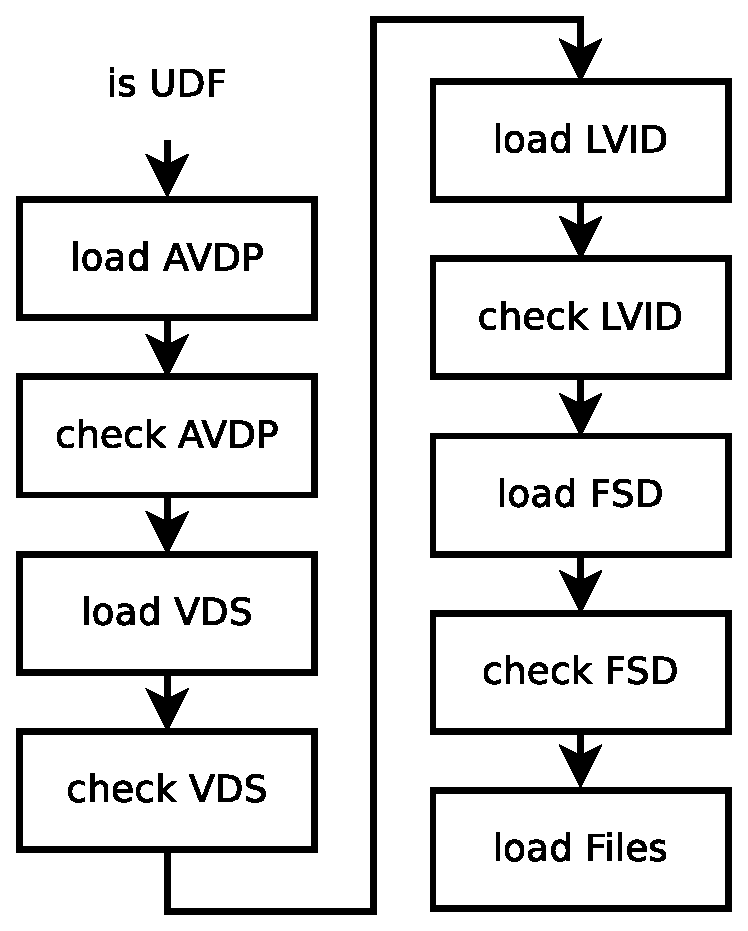
\includegraphics[scale=0.4]{obrazky/steps1.eps}
    \caption{Zjednodušený algoritmus činnosti programu}
    \label{fig:steps1}
\end{figure}

\section{Detekce chyb na médiu}
Detekce chyb na médiu je v tuto chvíli implementována pouze na úrovni porovnání kontrolních součtů a CRC.\\
Kontrolní součty jsou implementovány mou funkcí\\
\centerline{\texttt{\detokenize{uint8_t calculate_checksum(descTag tag)}}}\\
v souboru \texttt{udffsck.c}. Tato funkce pouze počítá checksum nad zadaným tagem a výsledek vrací. Proto je zapouzdřena do funkce\\ \todo{Doplnit kapitolu checksum}
\centerline{\texttt{\detokenize{int checksum(descTag tag)}}}\\
která přidává porovnání se checksum v tagu. Takto fukce vrací 0 při rozdílu a nenulovou hodnotu při shodě.\\
CRC je počítáno funkcí sdílené knihovny, která je součástí balíku. Ta byla opět zapouzdřena funkcí\\
\centerline{\texttt{\detokenize{int crc(void * desc, uint16_t size)}}}\\
aby vracela tentokrát 0 při neshodě a nenulovou hodnotu při shodě. Oproti funkci pro výpočet kontrolního součtu je třeba funkci pro výpočet CRC dodat i délku. Důvodem je, že \textit{DescriptorTag} má fixní délku a tu lze zjistit ze struktury, která jej popisuje pomocí funkce \texttt{sizeof}. Deskriptory ovšem tuto vlastnost nemají. Jsou deskriptory, které mají délku fixní, ale část má délku proměnnou podle dat, která nesou (například délka struktury \textit{File Entry} se závislá na tom, jestli se jedná o soubor nebo adresář a v případě adresáře ještě kolik dalších deskriptorů je uvnitř.)

\section{Oprava deskriptoru}
\label{sec:oprava-deskriptoru}
Oprava deskriptoru při detekci chyby pomocí kontrolních mechanismů CRC, kontrolní součet nebo špaté pozice v \textit{Tag Location} probíhá v šesti krocích. Předpokladem takové opravy je existence správného zdrojového deskriptoru nebo dostatek dat pro jeho znovuvytvoření. Kroky opravy jsou tyto:
\begin{enumerate}
    \item Určení pozic zdrojového (správného) deskriptoru a cílového (defektního) deskriptoru.
    \item Zkopírování zdrojového deskriptoru do paměti. Tímto vytvoříme nový cílový deskriptor.
    \item Opravení položky \textit{Tag Location} v tagu nového cílového deskriptoru podle pozice původního cílového deskriptoru.
    \item Výpočet CRC nad novým cílovým deskriptorem a uložení výsledku do tagu (Teoreticky nadbytečný krok, CRC by mělo být stejné jako u původního deskriptoru. Tento krok je užitečný pro vývoj kdy lze tímto oveřit, že byl zkorpírovaný celý zdrojový deskriptor.)
    \item Výpočet kontrolního součtu tagu nového cílového deskriptoru a uložení výsledku do tagu (Zde již je nutné kontrolní součet spočítat, protože se změnila pozice uložená v tagu podle nového umístění deskriptoru.)
    \item Zkopírování nového cílového deskriptoru na místo původního cílového deskriptoru.
\end{enumerate}

\section{Mapa chyb}
\label{sec:mapa-chyb}
Účelem takzvané mapy chyb (neboli struktury \texttt{\detokenize{vds_sequence_t}}) je zapouzdření chyb, které jsou detekovány napříč médiem v deskriptorech, vyjma chyb v deskriptorech dat. Její struktura je v tabulce \ref{tab:err-seq}.\\
Jak je vidět, je složena z malých struktur s názvem \texttt{\detokenize{metadata_t}}. Ty jsou popsány tabulkou \ref{tab:metadata-t}. Jak je vidět, obsahuje pouze identifikátor deskriptoru (použité pouze u VDS, více v kapitole \ref{sec:oprava-vds}), pozici deskriptoru a bitové pole chyb. Význam jednotlivých bitů je popsán v tabulce \ref{tab:E-codes}.
\begin{table}[hb]
    \begin{tabular}{ | l | l | p{2cm} | l | p{5.5cm} | }
        \hline
        Adresa  & Délka [B]   & Jméno položky & Datový typ & Popis \\ \hline
        0       & 21          & anchor         & pole \detokenize{metadata_t} \ref{tab:metadata-t} & Chyby v AVDP \\ \hline 
        21      & 56          & main           & pole \detokenize{metadata_t} \ref{tab:metadata-t} & Chyby v Hlavním VDS \\ \hline 
        77      & 56          & reserve        & pole \detokenize{metadata_t} \ref{tab:metadata-t} & Chyby v Záložním VDS \\ \hline 
        133     & 7           & lvid           & \detokenize{metadata_t} \ref{tab:metadata-t} & Chyby v LVID \\ \hline 
        140     & 7           & pd             & \detokenize{metadata_t} \ref{tab:metadata-t} & Chyby v PD \\ \hline 
    \end{tabular}
    \caption{Formát struktury \texttt{vds\_sequence\_t} (Mapa chyb)\label{tab:err-seq}}
\end{table}
\begin{table}[hb]
    \begin{tabular}{ | l | l | p{4.5cm} | p{1.3cm} | p{5.5cm} | }
        \hline
        Adresa  & Délka [B]   & Jméno položky & Datový typ & Popis \\ \hline
        0       & 2          & tagIdent       & Uint16     & Identifikátor deskriptoru \\ \hline 
        2       & 4          & tagLocation    & Uint32     & Pozice deskriptoru \\ \hline 
        6       & 1          & error          & Uint8      & Bitové pole nalezených chyb (tabulka \ref{tab:E-codes}) \\ \hline 
    \end{tabular}
    \caption{Formát struktury \texttt{metadata\_t}\label{tab:metadata-t}}
\end{table}
\begin{table}
    \begin{tabular}{ | l | l | l | }
        \hline
        Název & Maska & Význam \\ \hline
        \texttt{E\_CHECKSUM} & \texttt{0b00000001} & Chyba v konrolním součtu \\ \hline
        \texttt{E\_CRC}      & \texttt{0b00000010} & Chyba v CRC \\ \hline
        \texttt{E\_POSITION} & \texttt{0b00000100} & Chyba v umístění deskriptoru\\ \hline
        \texttt{E\_WRONGDESC}& \texttt{0b00001000} & Nenalezen očekávaný deskriptor (použito pouze pro AVDP)\\ \hline
        \texttt{E\_UUID}     & \texttt{0b00010000} & Chyba UUID souboru \\ \hline
        \texttt{E\_TIMESTAMP}& \texttt{0b00100000} & Chyba časové značky souboru\\ \hline
    \end{tabular}
    \caption{Chybové kódy pro strukturu \texttt{metadata\_t}\label{tab:E-codes}}
\end{table}

\section{Výstup a ovládání nástroje}
Nástroj \texttt{udffsck} je navržen po vzoru ostatních nástrojů z rodiny \texttt{fsck}. Tomu bude odpovídat i jeho ovládání a výstup.\\
Vstupy různých \texttt{fsck} nástrojů se liší podle jednotlivých souborových systémů, ale kvůli zapouzdřitelnosti musí dodržovat návratové hodnoty pro různé druhy chyb. Jedná se o tyto hodnoty:
\begin{itemize}
    \item 0 - Bez chyb 
    \item 1 - Opraveny chyby na souborovém systému
    \item 2 - Opraveny chyby na souborovém systému, doporučený reboot 
    \item 4 - Chyby souborového systému zůstaly neopraveny
    \item 8 - Chyba programu
    \item 16 - Chybné vstupní parametry
    \item 32 - Kontrola byla přerušena na základě uživatelského požadavku
    \item 128 - Chyba sdílené knihovny
\end{itemize}
Návratová hodnota může být i součet těchto hodnot pokud nastalo více chyb zároveň.\\
Má implementace v tuto chvíli nerespektuje tyto hodnoty z důvodů vývoje a vrací různé chybové kódy podle místa kde program skončil. Toto chování bude nahrazeno lepšími výpisy do standardního výstupu a chybového výstupu.\\
Jedná se o terminálový program bez jakéhokoli grafického uživatelského rozhraní nebo i textového uživatelského rozhraní. Běh programu je možné ovlivnit pouze jeho vstupními parametry, které jsou dodány při jeho spuštění spolu s médiem ke kontrole. Jeho výstupy jsou směrovány na standardní výstup \texttt{stdout} a chybový výstup \texttt{stderr}. V tuto chvíli není výstup programu sjednocený do uživatelsky přívětivé podoby ale spíše pro vývojáře, protože se vypisuje vysoké množství ladicích a informativních údajů.\\
Program v tuto chvíli vyžaduje k běhu informaci o velikosti sektoru média a médium samotné. Volání programu může vypadat například takto:\\ 
\centerline{\texttt{./udffsck -b 2048 medium.img}}\\
První je samotný program, poté následuje povinný parametr \texttt{-b} následovaný velikostí fyzického sektoru. Mezera mezi paramtrem a hodnotou není povinná. Posledním parametrem je samotné kontrolované médium. Jemu nepředchází žádný identifikátor.\\
Ukázkový výstup programu je v příloze \ref{lst:bs512} včetně komentáře jednotlivých částí výstupu. 

\section{Načtení média a jeho příprava na zpracování}
Životní cyklus média v mé implementaci začíná předáním cesty k médiu při spuštění programu. Ta musí vést přímo k zařízení jako takovému, nikoli k místu kam je připojeno.\\
Médium je na základě cesty načteno. Jednou pomocí funkce \texttt{open(2)} \ref{posix-open} pro práci samotnou, podruhé pomocí \texttt{fopen(3)} \ref{posix-fopen} pro nalezení velikosti média. Volání \texttt{fopen(3)} je pouze pro čtení, protože po úspěšném zjištění velikosti média není dále potřeba. Volání \texttt{open(2)} se liší podle dalších argumentů při spuštění programu. Pokud je médium pouze kontrolování, je médium otevřeno pro čtení. Pokud je požadována i korekce (ať už automatická nebo interaktivní), je otevřeno pro čtení a zápis.\\
Dalším krokem po načtení je zamčení média pomocí funkce \texttt{flock(2)} \ref{posix-flock}. Důvodem je zamezení paralelního přístupu k médiu při kontrole. Není žádoucí, aby médium mohlo být měněno během kontroly a korekce. Použití této funkce je implementováno jako neblokující. V případě nemožnosti uzamčít médium program skončí s chybou.\\
Po úspěšném zamčení média následuje namapování média do paměti funkcí \texttt{mmap(2)} \ref{posix-mmap}. Ta přebírá referenci na médium z funkce \texttt{open(2)} a stejně tak se liší její parametry podle požadavků na kontrolu nebo i korekci. Pokud je médium úspěšně namapováno do paměti, je možné přistoupit k práci s médiem jako takovým.\\
První otázka která vyvstává je duální otevření stejného souboru pouze pro zjištění velikosti média. Existuje funkce \texttt{fstat(2)} \ref{posix-fstat}, která slouží ke zjištění údajů o souboru a pracuje s referencí z volání \texttt{open(2)}. Tato funkce naplní strukturu \texttt{struct stat} a ta obsahuje údaje jako je velikost souboru nebo ideální velikost bloku. Problém je, že tato funkce selže při použití se surovým médiem (tímto je myšlen přístup přímo na úložiště přes cestu \texttt{/dev/sdX}). Pokud by program pracoval pouze s obrazy disků, které jsou uložené jako soubor na souborovém systému, použití této funkce by bylo ideální. Ovšem v tomto případě je nejpřijatelnější přístup načtení média znovu a použití funkce \texttt{fseeko(3)} \ref{posix-fseeko} s parametrem \texttt{SEEK\_END} a následně zjištění aktuální pozice funkcí \texttt{ftello(3)} \ref{posix-ftello}. Důvodem použití \texttt{fseeko(3)} a \texttt{ftello(3)} místo \texttt{fseek(3)} \ref{posix-fseek} a \texttt{ftell(3)} \ref{posix-ftell} je návratový typ \texttt{off\_t}, který narozdíl od \texttt{long} neumožňuje záporné hodnoty, tudíž je použití těchto funkcí preferované v nových projektech.\\
Druhá otázka vyvstává u použití funkce \texttt{mmap(2)} a výhodám oproti funkcím \texttt{read(2)} \ref{posix-read} a \texttt{write(2)} \ref{posix-write}. Důvodů je několik, počínaje pohodlností použití. Pokud je soubor mapovanán do paměti, je s ním z hlediska programu pracováno jako s jednorozměrným polem o velikosti mapovaného souboru. Tím pádem lze přistupovat na libovolné místo souboru bez nutnosti používat \texttt{lseek(2)}, lze snadno referencovat kusy souboru do struktur a poté s ním pracovat ve struktuře místo nutnosti ho do struktury kopírovat. Rizikem tohoto přístupu je setření hranice mezi médiem a operační pamětí a tudíž opatrnost při zápistu zpět do média aby nedošlo k nežádoucí modifikaci souboru.

\section{Kontrola přítomnosti souborového systému UDF}
Po úspěšném načtení média je prvním krokem před jakoukoli další prací kontrola přítomnosti správného souborového systému, v tomto případě UDF. Tato kontrola probíhá kontrolou oblasti \textit{Volume Recogniton Sequence} (VRS) pomocí funkce \texttt{is\_udf()}. Tato funkce načte blok na sektoru 16. Tento blok je fixní místo na souborovém systému a je shodný pro UDF a ISO~9660, který je přímý předchůdce UDF. Zvláštností načítání VRS je velikost sektoru. Z důvodu zachování kompatibility s ISO~9660, který podporuje pouze velikost bloku 2048~B je tato velikost převzata jako konstanta, nezávisle na skutečné velikosti bloku média. Ovšem i tento axiom má výjimku a to že toto platí pouze do velikosti bloku 2048~B. Na médiích s větší velikostí bloku je již použita skutečná velikost bloku místo 2048~B. To je možné díky skutečnosti, že ISO~9660 nikdy nebude možné použít na takovém médiu. U médií s menší velikostí bloku by ISO~9660 stále použít šlo, stačí pouze zapisovat na více bloků místo jednoho při zápisu 2048~B.\\
Kontrola samotná probíhá načtením struktur VRS kde se vyhledávají deskriptory popisující UDF, t.j. deskriptory obsahující identifikátor \texttt{NSR01}, \texttt{NSR02} nebo \texttt{NSR03}. Pokud je takovýto identifikátor nalezen, a spolu s ním je i nalezen identifikátor \texttt{TEA01} (\textit{Terminating Extended Area}) je médium prohlášeno za správné a může se přistoupit ke kontrole. Pokud je nalezena identifikace UDF ale ne kompletní \textit{Extended Area}, může to znamenat neuzavřené médium a to pro další kontrolu znamená jiné umístění AVDP. Kontrola je ale možná. Pakliže nebyl nalezen identifikátor UDF, kontrola končí chybou a program končí protože nebylo možné detekovat přítomnost UDF.\\
Druhou činností, kterou funkce \texttt{is\_udf()} pokrývá je první pokus o detekci velikosti sektoru. Ta postupně zkouší načíst platné deskriptory pro různé povolené velikosti sektoru (hodnoty dělitelné beze zbytku 512, v praxi ovšem pouze omezená řada 512, 1024, 2048, 4096~B) a ukládá hodnotu kdy se to podaří. Prakticky by se to mělo podařit pouze pro velikost sektoru 2048~B a 4096~B. Pro velikosti sektoru média 2048~B včetně je obvykle detekovaná velikost sektoru 512~B (neboli nejnižší možná). S touto hodnotou poté dále pracuje detekce AVDP, která ji používá jako výchozí bodu svého hledání velikosti sektoru.

\section{Načtení, kontrola a korekce AVDP}
\todo{Popsat variantu unclosed and closed medium}
AVDP je klíčovou částí UDF, protože určuje výchozí bod pro čtení souborového systému. Jak je uvedeno v kapitole \ref{sec:avdp}, UDF rozlišuje čtyři možná umístění AVDP, přičemž přítomny mohou být až tři na médiu.\\
Jejich načítání pro potřeby další práce se souborovým systém lze popsat algoritmem na obrázku \ref{fig:avdp}. Algoritmus prochází možné lokace AVDP dokud neuspěje nebo nedojdou možnosti. Pro potřeby kontroly a opravy média je třeba po nalezení alespoň jednoho správného AVDP ostatní podle něj opravit.
\begin{figure}[ht] 
    \centering
    %\resizebox{0.5\textwidth}{!}{\input{obrazky/avdp.tex}}}
    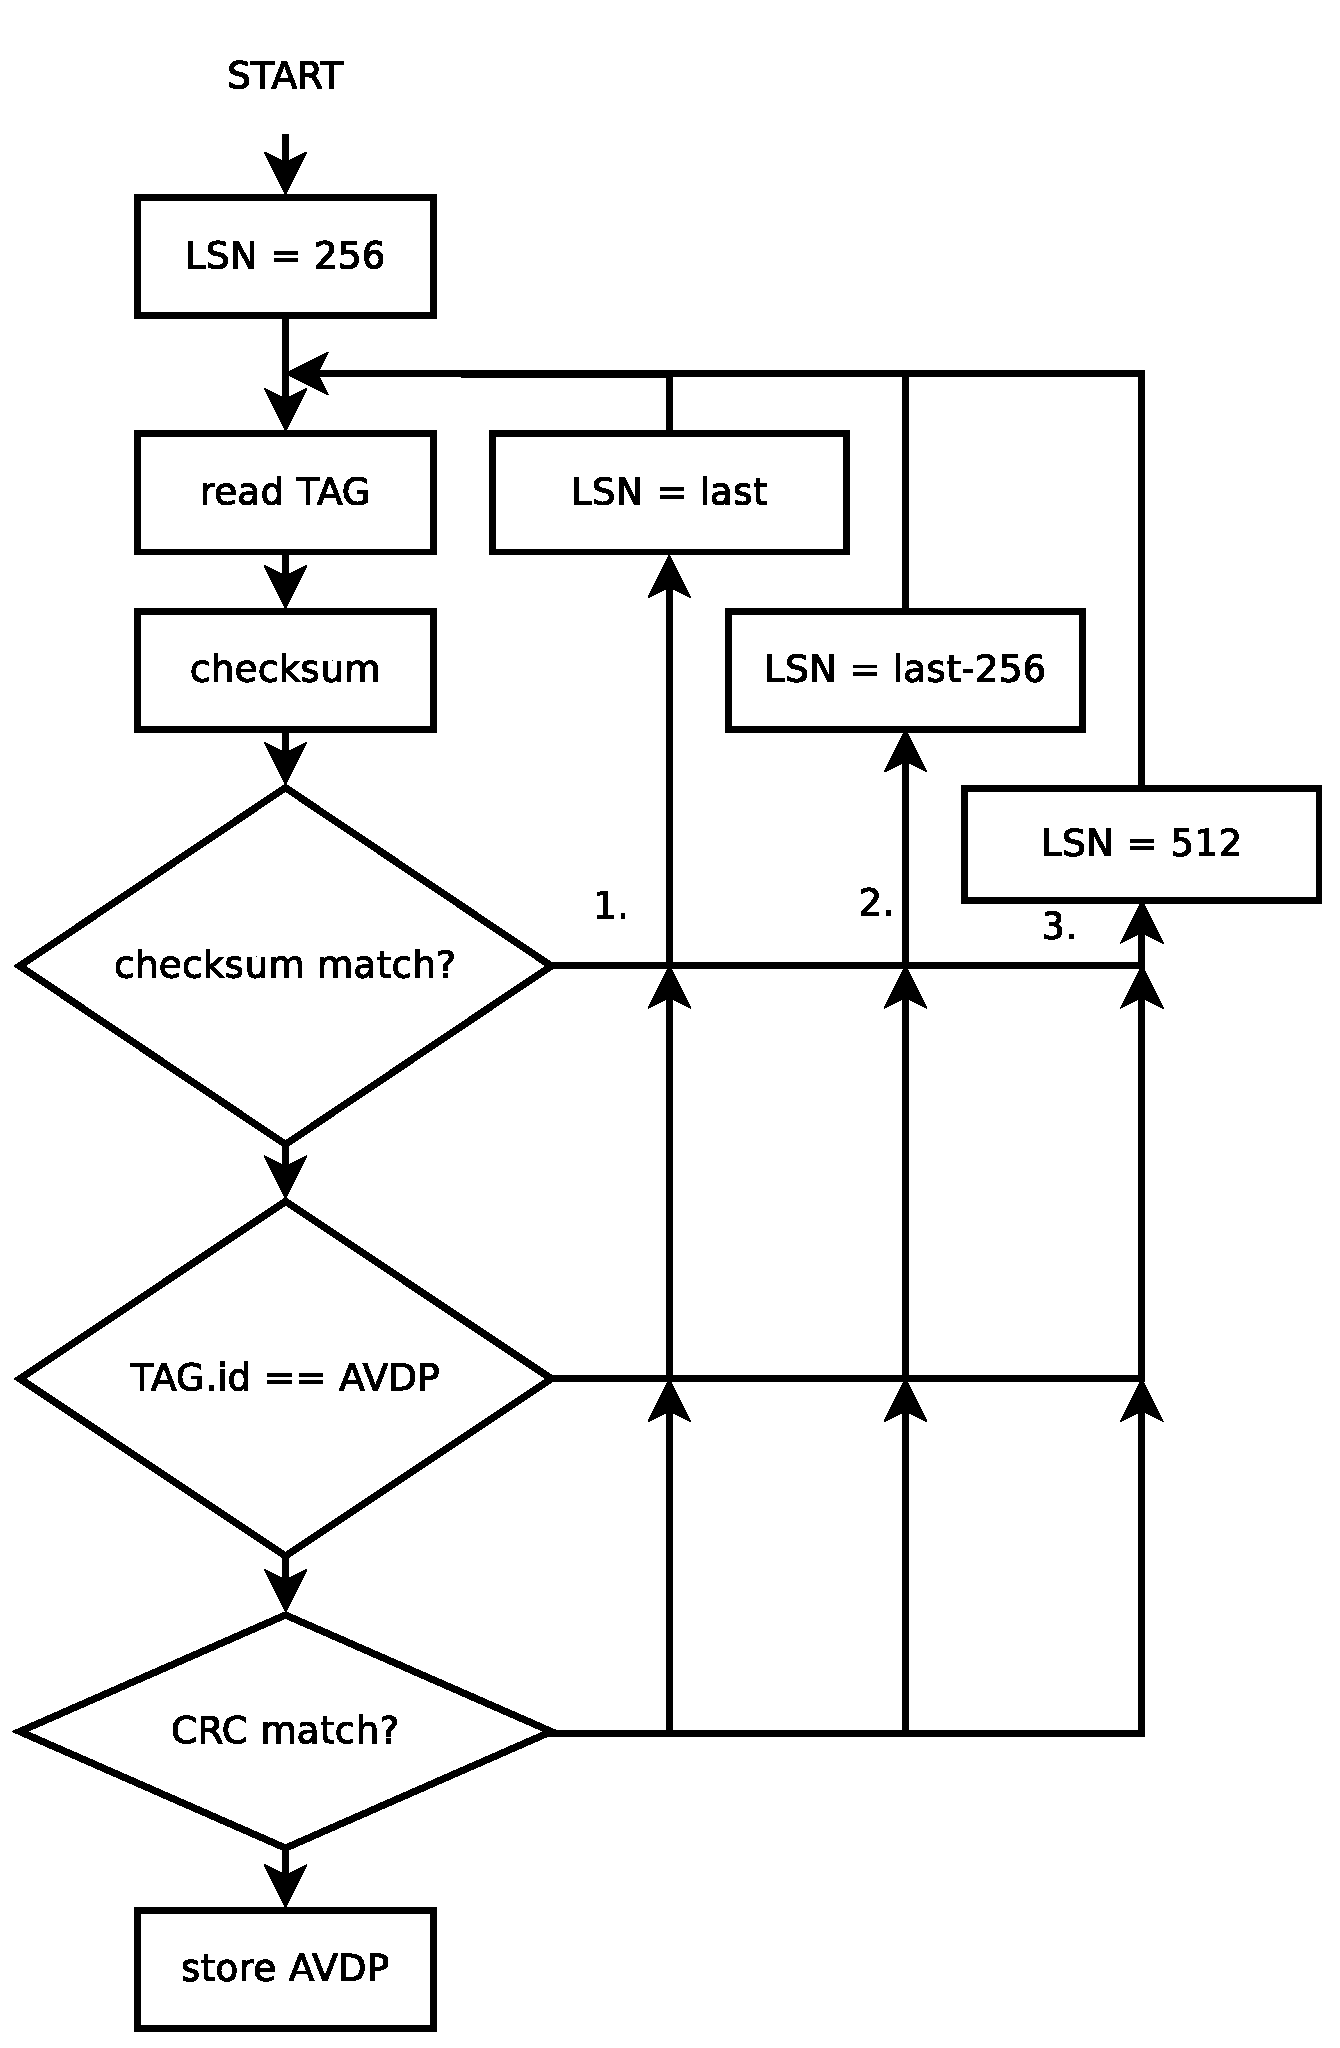
\includegraphics[scale=0.4]{obrazky/avdp.eps}
    \caption{Zjednodušený algoritmus načtení AVDP}
    \label{fig:avdp}
\end{figure}
\todo{Korekce AVDP}
\label{sec:oprava-avdp}
Oprava AVDP je možná pouze na uzavřených médiích. Důvodem je požadavek opravného algoritmu na přítomnost alespoň jednoho nepoškozeného (správného) deskriptoru, který bude použit jako vzor pro opravu. Otevřená (neukončená) média mají pouze jeden AVDP, proto v případě jeho poškození není oprava snadno možná.\\
Poté, co jsou nalezeny AVDP na svch pozicích (t.j. sektoru 256 a na posledním sektoru, případně na sektoru 512) a je určeno, který z nich je poškozený a který je v pořádku lze přistoupit k opravě, pokud je alespoň jeden v pořádku.\\
Samotný opravný algoritmus je popsán v kapitole \ref{sec:oprava-deskriptoru}.\\
Případné nalezené chyby jsou uloženy do struktur popsaných v kapitole \ref{sec:mapa-chyb}.\\

\section{Načtení, kontrola a korekce VDS}
Po úspěšném nalezení funkčního AVDP je možné načíst \textit{Volume Descriptor Sequence} (VDS). Tato skupina metadat je uložena na dvou místech, typicky jedno na začátku a druhé na konci média. Pozice obou je uložena právě v AVDP.\\
Tato skupina deskriptorů je popsána v kapitole \ref{sec:vds}. Deskriptory jsou uloženy za sebou v jednotlivých sektorech, přičemž poslední musí být vždy \textit{Terminating Descriptor}. Jak hlavní, tak záložní VDS by měly být ekvivalentní.\\
Jednotlivé deskriptory jsou načítány a ukládány do struktur pro další zpracování. První kontrola během načítání spočívá v porovnání kontrolního součtu tagu deskriptoru. Pokud tato kontrola uspěje, je možné provést porovnání CRC, protože již máme díky ověřenému tagu jistou totožnost deskriptoru, jeho předpokládané CRC a polohu. Pokud kontrola CRC uspěje, zkontroluje se poloha deskriptoru vůči deklarovanému umístění v tagu. Pokud i tato kontrola je v pořádku, lze prohlásit tag za správný. Pokud by byly v pořádku jako kontrolní součet, tak CRC, ale bylo by špatně deklarované umístění, lze s tagem pracovat, protože data která nese jsou s největší pravděpodobností v pořádku, ale je nutné opravit jeho umístění a následně přepočítat kontrolní součet a CRC. 

\todo{Korekce VDS}
\label{sec:oprava-vds}
Oprava \textit{Volume Descriptor Sequence} je podobná jako oprava AVDP. Předpokladem úspěšné opravy je opět existence alespoň jednoho správného zdrojového deskriptoru od každého typu, který ve VDS je. Pokud je toto splněno, je oprava možná.\\
Algoritmus je navržen takto:
\begin{enumerate}
    \item Během načítání VDS (jak hlavního, tak záložního) je vytvářena mapa chyb na jednotlivých deskriptorech. Formát mapy je popsán v tabulce \ref{tab:err-seq}. 
    \item Na základě údajů mapy chyb je přistoupeno o opravě. Pokud je alespoň jeden z deskriptorů v pořádku, je použit algoritmus z kapitoly \ref{sec:oprava-deskriptoru}. Pokud ne, je vypsána chyba a pokračuje se k dalšímu deskriptoru.
    \item Krok 2 se opakuje dokud není nalezen \textit{Terminating Descriptor}. Poté je oprava ukončena, protože byl nalezen konec VDS.
\end{enumerate}

\section{Načtení, kontrola a korekce LVID}
\label{sec:nacteni-a-kontrola-lvid}
\textit{Logical Volume Integrity Descriptor} (LVID) je důležitou částí UDF. Je umístěné mimo VDS a jeho pozice je uložena v LVD pod položkou \textit{Integrity Sequence Extent}. LVID není redundantní, což zjednodušuje práci s ním, ale zároveň se kvůli tomu jedná o slabé místo UDF. Ovšem je potřeba vzít v potaz skutečnost, že LVID lze v případě nepoškozeného souborového systému vytvořit znovu zpětně. V případě poškozeného souborového systému jej lze vytvořit též, ale s rizikem ztráty dat z důvodu nekompletní informace o souborovém systému v jiných deskriptorech.\\
Po kontrole kontrolního součtu a CRC je přistoupeno k samotnému načtení dat. Pro snažší práci s daty uloženými v LVID jsou data ukládána do struktury \texttt{filesystemStats}. Protože nadřazeným standardem je ECMA-167, jsou struktury popsány podle ní. Ovšem samotnou implementací je UDF standard a ten využívá pole \textit{Implementation~Use}, kam ukládá tyto údaje:
\begin{itemize}
    \item Počet souborů na svazku
    \item Počet adresářů na svazku
    \item Minimální revize UDF, se kterou je možné médium číst
    \item Minimální revize UDF, se kterou je možné na médium zapisovat
    \item Maximální revize UDF, se kterou je možné na médium zapisovat
\end{itemize}
Podobná situace je u položky \textit{Logical Volume Contents Use}. UDF tuto položku používá k uložení \textit{Logical Volume Header Descriptor}, což je struktura popsaná pomocí standardu ECMA-167 s jediným cílem a tím je uložení dalšího \textit{Unique ID}, neboli unikátního identifikátoru, který nese každý soubor a adresář na médiu. Význam \textit{Unique ID} je popsán v kapitole \ref{sec:filetree}.\\
Další částí je \textit{Free Space Table}, což je tabulka obsahující informaci o velikosti logického svazku a volného místa na něm. Oba údaje jsou v logických blocích, nikoli v bytech.\\
Důležitou částí je i časová značka poslední modifikace logického svazku. Tato značka, uložené v UTC, by mělo být vždy nejnovější ze všech časových značek na svazku.\\
Poslední položkou, která je důležitá pro prácí se svazkem je \textit{Integrity Type}. Ten může být buď otevřený (\textit{Open}) nebo uzavřený (\textit{Close}). Princip otevřeného a uzavřeného média je popsán v kapitole \ref{sec:kontrolni-mechanismy}. Pokud je uzavřený, tak by měl být svazek v konzistentním stavu. Pakliže je otevřený, je možné že probíhá zápisová operace, nebo že byl svazek během ní nesprávně odebrán. Tento indikátor pomáhá vyvolat požadavek na kontrolu média v operačním systému a pro kontrolu to je důležitý ukazatel upozorňující na pravděpodbnou nesrovnalost mezi deklarovaným volným místem a skutečností. 

\todo{Korekce LVID}
\label{sec:oprava-lvid}
Korekce LVID je odlišná od ostatních korekcí z důvodu absence redundantního LVID. Z toho vyplývá, že LVID nelze v případě poškození jako takového opravit. LVID ale obsahuje důležité informace o konzistenci média jako takového (viz kapitola \ref{sec:lvid}) a proto je korekce soustředěna na ně.\\
Opravují se tyto položky:
\begin{itemize}
    \item Vyvolání opravy SBD (kapitola \ref{sec:oprava-sbd})
    \item Počet souborů a složek.
    \item Následující \textit{Unique ID}.
    \item Datum posledního záznamu se nastaví na čas opravy.
    \item Opraví se tabulka volného místa \textit{Free Space Table}.
    \item Médium se uzavře (\textit{Integirty type} se nastaví na \textit{Closed}).
    \item Přepočítá se kontrolní součet a CRC.
\end{itemize}
Korekce je spouštěna z několika různých důvodů, které sice ve většině případů nastávají současně, ale mohou se vyskytnout i odděleně. Jedná se o tyto zdroje:
\begin{itemize}
    \item Pokud bylo nalezeno \textit{Unique ID} stejné nebo větší jako uloženo v LVID.
    \item Pokud byl nalezen soubor s novějším datem než je datum posledního záznamu v LVID.
    \item Pokud byla nalezena nesrovnalost v počtu souborů nebo složek uložených v LVID vůči skutečnému počtu.
    \item Pokud byl \textit{Integrity Type} ponechán ve stavu \textit{Open}.
\end{itemize}




\section{Korekce SBD}
\label{sec:oprava-sbd}
\textit{Space Bitmap Descriptor} je deskriptor popisující volné a obsazené místo na logickém svazku z hlediska umístění jednotlivých bloků. Jedná se o vektor bytů (\textit{Bitmap}) o délce $PocetLBN / 8$. Spolu s ním je uložena jeho délka (\textit{Number of Bytes}) a skutečný počet bloků (\textit{Number of Bits}).\\ 
Každý jeden byte v tomto vektoru odpovídá osmi logickým blokům v přirozeném pořadí (nejméně významný bit odpovídá prvnímu bloku, nevíce významný bit odpovídá osmému bloku).\\
Hodnota bitu označuje stav bloku. Logická 1 odpovídá volnému bloku, logická 0 obsazenému bloku. Přebývající bity v posledním bytu se označují jako obsazené.\\
Korekce probíhá tak, že během průchodu souborovým stromem se vytváří nový vektor obsazenéhé místa o stejné velikosti jako původní. Ten slouží jako referenční mapa, která bude nakopírována na místo původní v případě nutnosti opravy.\\
Oprava je vyvolána automaticky při opravě LVID (kapitola \ref{sec:oprava-lvid}), při rozdílu počtu použitých bloků oproti počtu ve vektoru nebo pokud při načítání došlo k chybě v kontrolním součtu nebo CRC.



\section{Kontrola a obnova stromu souborů}
\label{sec:filetree}
Obnova stromu uživatelských dat je klíčová část programu. Bez ní nemá tento nástroj význam. Vzhledem k faktu, že \texttt{fsck} nemá za cíl detekovat chyby v datech samotných a UDF také neimplementuje ochranné algoritmy na data samotná ale jen na metadata, není bohužel možné poškozená data ani detekovat, ani tudíž obnovit. Je možné se pokusit zrekonstruovat adresářovou strukturu a určit místo, kde by data měla být.\\
Algoritmus načtení adresářové struktury je zachycen na obrázku \ref{fig:files}. Tento algoritmus začíná po úspěšném načtení FSD, odkud je získána pozice FE kořenového adresáře (proto algoritmus začíná čtením FE). Pokud je toto úspěšné, pokračuje se k čtení FID a takto se postupně projde celou strukturou.\\
Místa na obrázku označená jako \textit{ERROR} značí místa, kde došlo k chybě některého z kontrolních mechanismů a bylo by nutné přistoupit k obnově. 
\begin{figure}[ht] 
    \centering
    %\resizebox{0.5\textwidth}{!}{\input{obrazky/avdp.tex}}}
    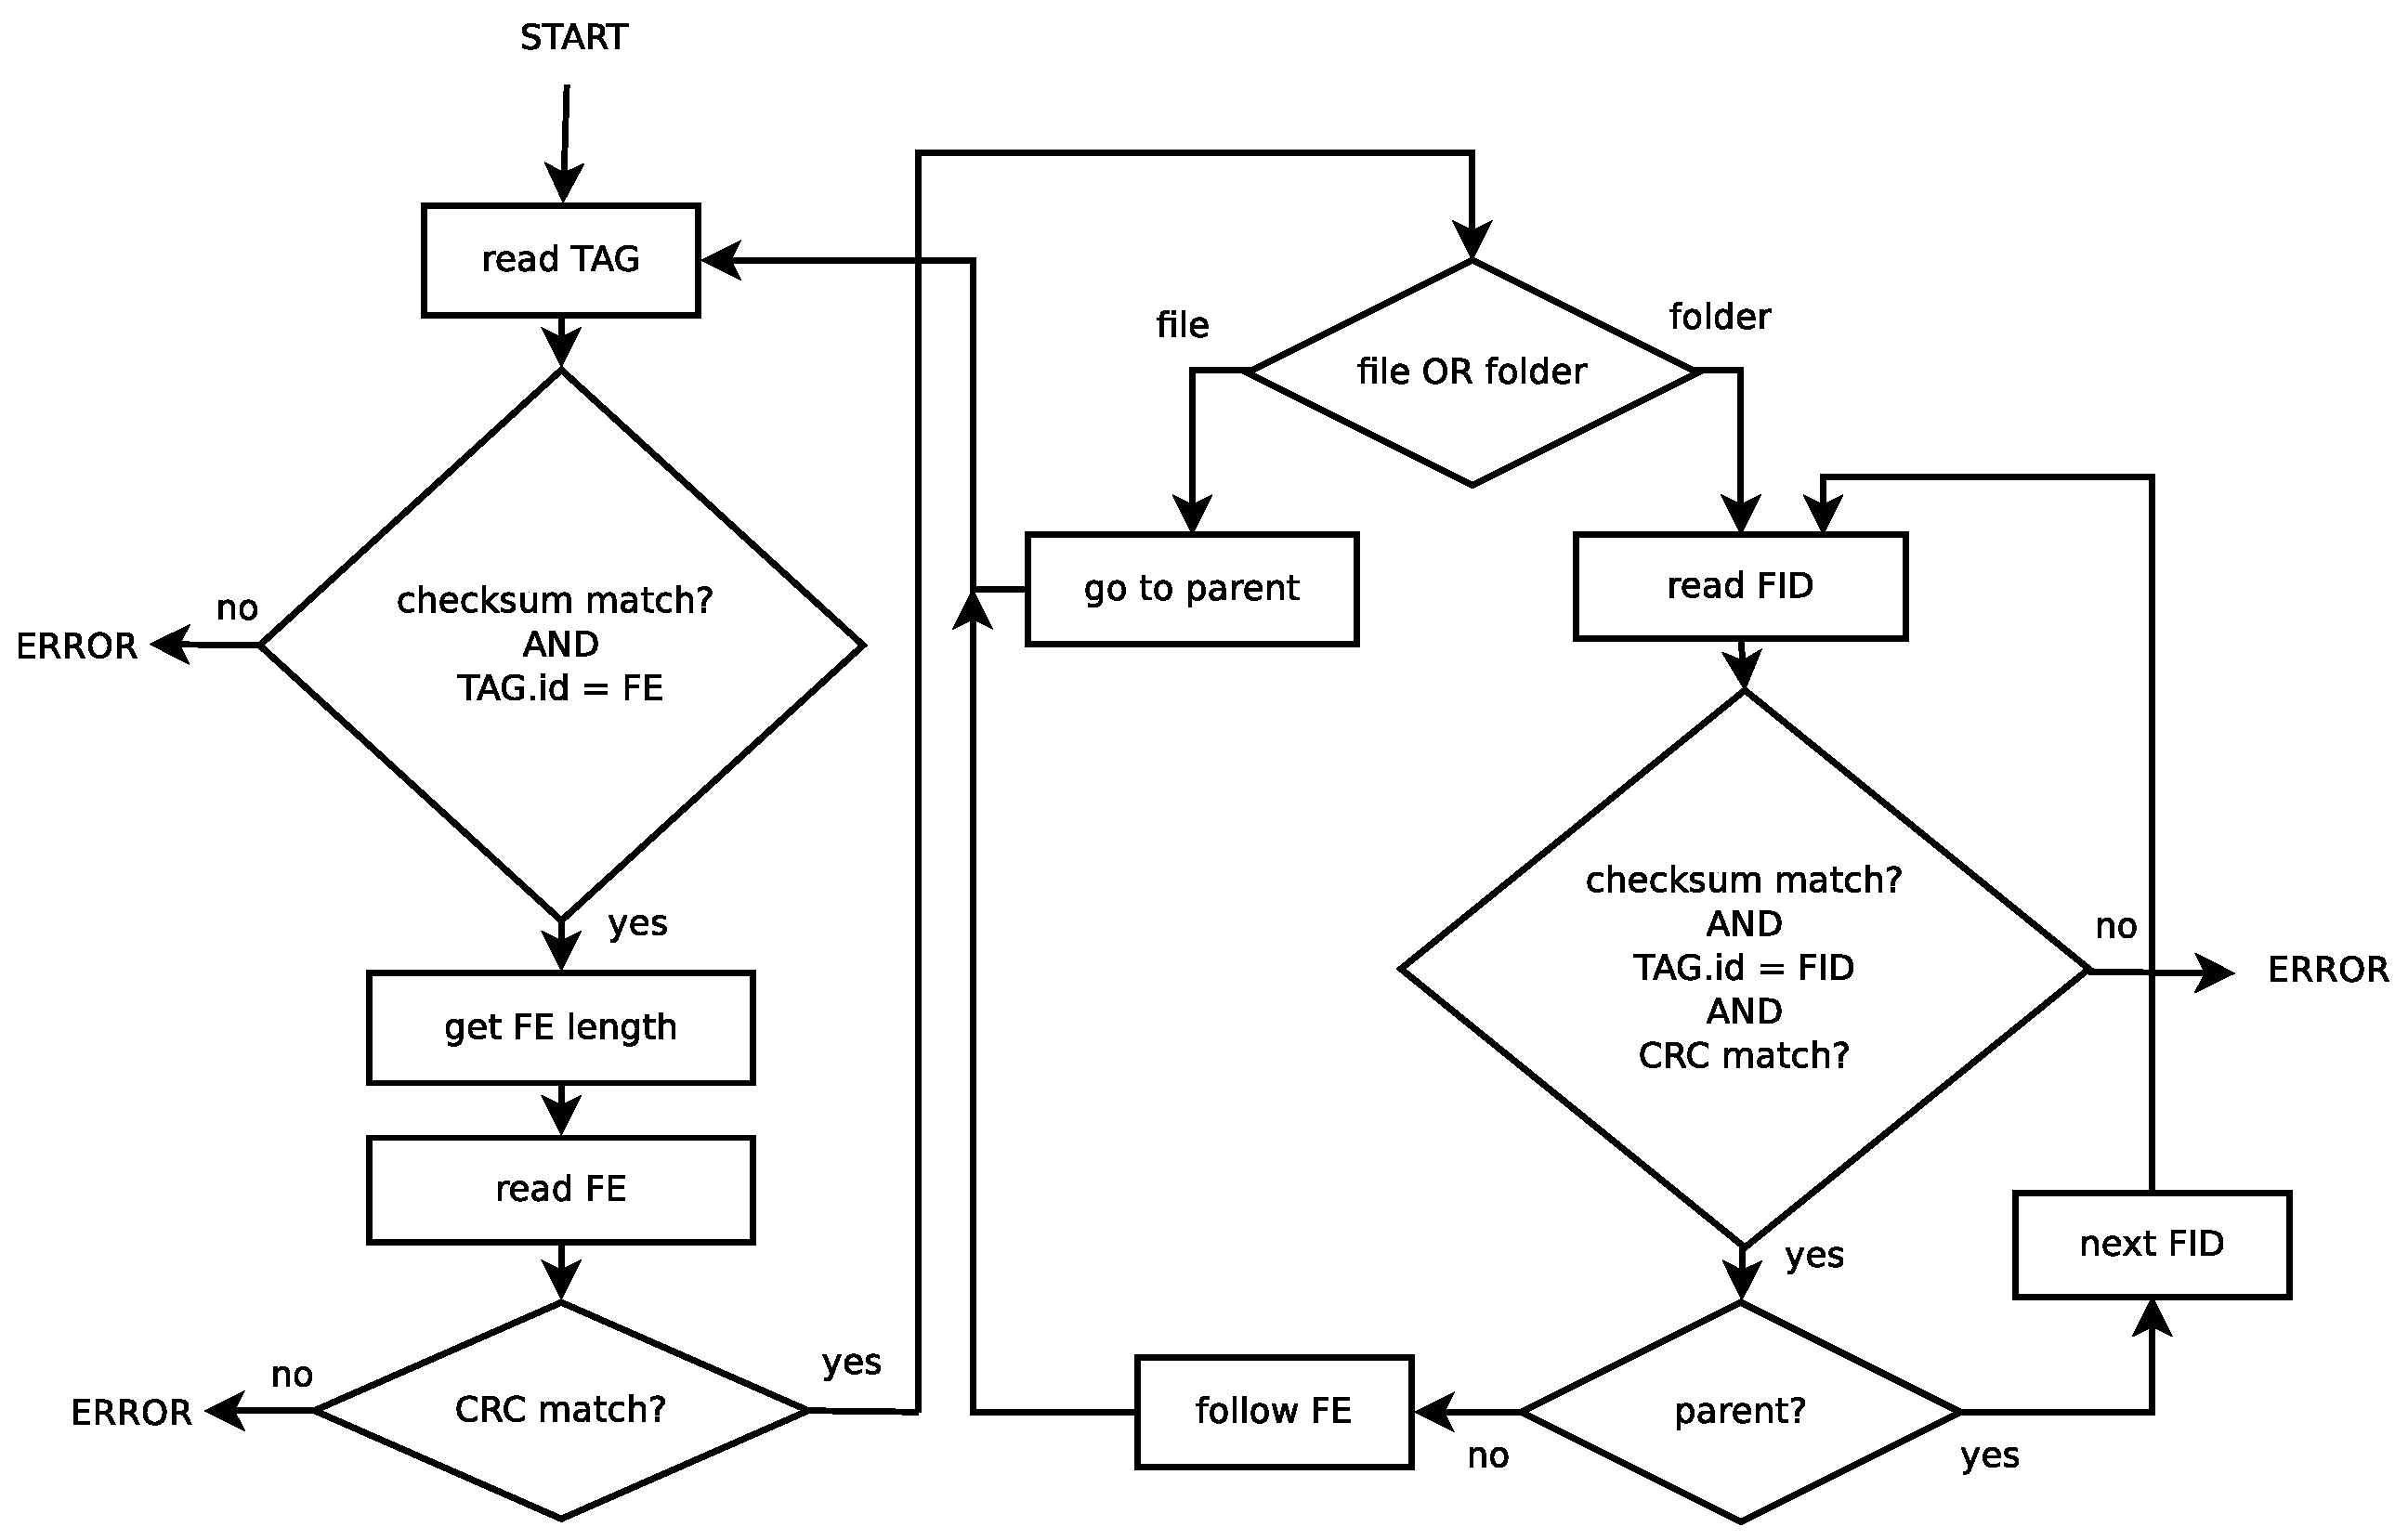
\includegraphics[scale=0.36]{obrazky/files.eps}
    \caption{Algoritmus načítání souborů}
    \label{fig:files}
\end{figure}
Během průchodu se sleduje několik parametrů, které jsou nutné ať už pro kontrolu a opravu stromu nebo pro opravu metadat v LVID \ref{sec:oprava-lvid} a SBD \ref{sec:oprava-sbd}. Jedná se o tyto:
\begin{itemize}
    \item Je \textit{Unique ID} nenulové (nulové musí být pouze pro \textit{root})?
    \item Je \textit{Unique ID} shodné pro FE a FID?
    \item Je \textit{Unique ID} menší než hodnota uložená v LVID?
    \item Jaký je čas poslední změny? Je tento čas později než je čas uložený v LVID? 
\end{itemize}
Pokud je kterýkoli dotaz zodpověděn záporně, je nastaven příznak chyby.\\
Několikrát zmiňovaný je parametr \textit{Unique ID}. Jedná se o příznak, který je unikátní pro každý soubor nebo adresář. Je stejný pro FE a FID. Důvodem je šance na obnovu v případně katastrofického poškození souborového stromu. Pokud by se muselo přistoupit ke hledání jednotlivých FE ve všech sektorech logického svazku a párovat je s FID v adresářích, toto by byla jediná šance na obnovu.\\
Základním předpokladem pro použití tohoto algoritmu je ztráta některého z adresářů (například kořenového adresáře). To způsobí nemožnost načíst strom souborů z důvodu chybějícího vstupního bodu do stromu souborů. Nutno podotknout, že tento algoritmus není zahrnut v implementaci, ale jeho myšlenková struktura je následující:
\begin{enumerate}
    \item Díky známé velikosti logického bloku a známému umístění deskriptorů v nich (vždy na jeho začátku) lze procházet logickým svazkem po blocích a na každém se pokusit načíst \textit{File Entry} (FE) nebo \textit{Extended File Entry} (EFE), verifikovat jeho platnost pomocí jeho polohy, CRC a kontrolního součtu.
    \item Takto nalezený seznam FE a EFE bude vytvářet samostatné podstromy souborů (pokud médimu obsahovalo další adresáře) a zbylé soubory bez rodičovského adresáře. Tato část probíhá podobně jako procházení stromem souborů, zkráceně takto:
    \begin{enumerate}
        \item Každý nalezený FE nebo EFE je klasifikován jako soubor nebo adresář. Pokud se jedná o adresář, je prohledán pro přítomnost \textit{File Identifier Descriptor} (FID). Pokud jsou nalezeny, dojde k pokusu spárovat je podle \textit{Unique ID} s ostatními nalezenými FE a EFE. Každý takto spárovaný FE (EFE) je vyřazen ze seznamu nalezených FE (EFE) a je zařazen do podstromu. Pokud se jedná o soubor, neděje se nic a pokračuje s k dalšímu nalezenému FE (EFE).
        \item Takto se vytvoří struktura podstromů a zbytku nezařazených FE a EFE.
    \end{enumerate}
    \item Nyní máme části původního stromu a zbytek FE (EFE). Ať už kořeny jednotlivých podstromů (nejvyšší adresář) nebo osamocené FE (EFE). Ty už není možné dále zařadit, proto budou zařazeny do chybějícího adresáře, který bude znovu vytvořen na místě původního. Jsou zde ovšem jistá omezení. Obnova není schopná zpětně získat názvy jednotlivých FE (EFE), protože ty jsou uloženy ve FID rodičovského adresáře. Stejně tak pokud by bylo nenávratně ztraceno více adresářů, nebylo by možné rozlišit, které FE (EFE) patří do kterého. 
\end{enumerate}
Jak je vidět ve výše popsaném algoritmu, obnova není absolutní, ale může poskytnout dobrý výchozí bod pro záchranu dat. 
